\section{Introduction}
%\subsection*{Performance models are important}
Most software systems can be customized via configuration options to meet user demands. The selection of configuration options can enable desired functionality (features) or tweak non-functional aspects of a software system, such as improving performance or energy consumption. 
All too often, software performance bugs can be linked to configuration options~\cite{han_empirical_2016}. 
The relationship of configuration choices and their influence on non-functional properties has been extensively studied in recent years. Most work focuses on the prediction of non-functional properties\footnote{In this paper, we use the terms \textit{non-functional properties} and \textit{performance} interchangably, although the latter term is more restricive. In the context of this work a performance model describes any model that predicts a non-functional property.}, such as execution time or memory utilization, for arbitrary configurations~\cite{dorn2020,siegmundPerformanceinfluenceModelsHighly2015,haDeepPerf2019,perfAL,guoVariabilityawarePerformancePrediction2013,sarkarCostEfficientSamplingPerformance,guo_2018_data,fourier_learning_2015,perLasso} or on finding configurations that are near-optimal with regard to a non-functional property~\cite{nairUsingBadLearners2017,nairFlash18,ohFindingNearoptimalConfigurations2017}. 
The backbone of performance estimation is a model that maps a given configuration to the estimated performance value. 
%In general, performance prediction models are only useful to practitioners if predictions hold for a large number of application scenarios.

%\subsection*{Performance models can be workload-biased}
{\color{olive}\todo{kürzen}
Learning performance models usually relies on a training set of configuration-specific performance measurements. 
Typically, established approaches employ only a single workload (e.g., a benchmark or test suite) to measure performance, which usually aims at emulating a specific real-world application scenario. 
However, as the collected measurements represent only the one application scenario, the resulting performance model can  estimate performance for this single scenario reliably. 
The choice of a single workload can introduce bias as the predictive model is only as useful as the underlying workload resembles a wide range of use cases in the real world. 
\citeauthor{alves_sampling_2020} illustrate this fact with an analysis of the video encoder \textsc{x264} under different workloads~\cite{alves_sampling_2020}. 
For two different workloads, they observed vastly different performance distributions across a large set of configurations.
While this particular observation might be the exception, in general, one cannot assume that performance behavior under a single workload is generalizable, and therefore consistent in every real-world setting.
In this vein, a recent exploratory study by \citeauthor{jamishidi_transfer_2017}~\cite{jamishidi_transfer_2017} illustrates that performance models of a configurable software system often exhibit differences in estimated performance influences when learned in different environments, including different versions, hardware setups, and workloads.
Performance  influences across different environments remain largely congruent and differences only affect small numbers of configuration options, such that differences can be learned efficiently via transfer learning~\cite{jamshidi_transfer_gp_2017,jamshidi_learning_2018}. 
Nonetheless, under a single workload, we are left with performance models whose estimations are potentially inaccurate for different environments. A specific workload might miss some lines of code and, hence, it is impossible to get performance information about such code regions.
}

%\subsection*{Towards Estimating Representativeness}

{
	\todo{MOtivation, konkretres Problem: Repräsentativität wenig untersicht}
\color{green}
Given not one, but a set of performance models based on different workloads, the question arises: Which performance model of the set is most general, whose estimations are more likely to \emph{represent} real-world scenarios? 
To assess which model's estimations to trust most, we require information about whether and how different workloads interact with the software system under test. 
}

{\color{red}
	\todo{Beschreibung von Listing 1 (code abhängig von OPtion sowie von Option und Workload), spiegelt sich ebenfalls in den Performance-Einflüssen wieder, daher: Workload matters}
Take as an example the method in Listing~\ref{lst:intro} from an imaginary database system. It receives as an argument an array of strings, each a row to insert. The method exhibits two configuration options, of whose selection some code sections depend: if \texttt{DUPLICATE\_CHECK} is enabled, the passed array is checked for duplicates via a separate method invocation (lines 2--4), and if \texttt{AUTOCOMMIT} is enabled, each insertion is treated as a single transaction (lines 10--12). The latter section, however, not only depends on the selection of a configuration option, but also on the number of rows to insert. If the workload (here, the number of rows) is large enough, the individual insertion per row (line 9) is replaced by another insertion method (line 6). This example illustrates, how the execution of a program could depend on both configuration decisions (lines 2--4) and workloads (lines 5--9), or interactions between them (lines 10--12).

\begin{figure}
\begin{subfigure}[l]{0.63\linewidth}
	
\lstinputlisting[caption=Workload-dependent code ,escapechar=\%,label=lst:intro]{examples/introduction.cc}

\end{subfigure}
	\begin{subfigure}[l]{0.35\linewidth}
		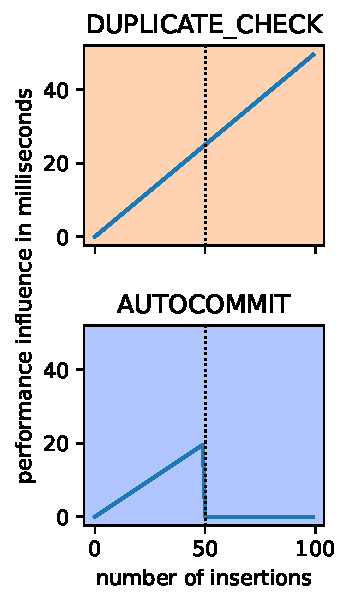
\includegraphics[width=1\linewidth]{images/influences.pdf}
	\end{subfigure}
	\caption{Illustrative example (left) with workload-dependent performance influences of configuration options \texttt{DUPLICATE\_CHECK} and \texttt{AUTOCOMMIT} (right).}
	\label{fig:intro}
\end{figure}


To now representatively assess the method's performance, one would require not only observations under a set of sample configurations, but also under different workloads to cover and measure performance for workload-dependent code. If dependent code, such as the interaction between \texttt{AUTOCOMMIT} and the workload size is missed, the estimation of an option's performance influence becomes unrepresentative and, thus, the performance model unreliable.
}

%\subsection*{Approach, Results \& Contribution}
{\color{blue}
	\todo{Haupt-Vorgehen und konkrete Ergebnisse}
In this paper, we explore how the selection of a workload can influence performance models how prone these are to be distorted. To this end, we extend our perspective from pure black-box measurements~\cite{dorn2020,siegmundPerformanceinfluenceModelsHighly2015,haDeepPerf2019,perfAL,guoVariabilityawarePerformancePrediction2013,sarkarCostEfficientSamplingPerformance,guo_2018_data,fourier_learning_2015,perLasso} with knowledge about the code executed. Specifically, we enrich performance measurements from different configurations under varying workloads with corresponding easy-to-compute code coverage data. 
We conduct an empirical study of seven configurable software systems to explore how the selection of workloads can influence both performance and code coverage, and possibly distort performance models (cf. Section~\ref{sec:study}). {\color{teal}We found that \ldots.} 
Based on our findings, we explore correlations between code coverage and differences in performance influence (Section~\ref{sec:metric}). 	We found that \ldots. We propose to use code coverage as a \ldots and devise a novel method to interpret performance model with regard to code coverage in order to estimate their representativeness.
}

In summary, we offer the following contributions:
\begin{itemize}

	\item An empirical study of X configurable software systems with a total number of Y configurations and Z workloads.
	\item A companion Web site\footnote{\url{https://github.com/icse-submitter123/submission}} providing supplementary material including performance measurements, code coverage data, and additional visualizations.
\end{itemize}

\section{Background and Related Work}
\subsection{Performance Prediction Modeling}
Configurable software systems are an umbrella term for any kind of software system that exhibits configuration options to customize functionality. 
While the primary purpose of configuration options is to select (categorical or binary options) and tune (numerical options) functionality, each configuration choice may also have implications on non-functional properties---be it intentional or unintentional. Finding configurations with optimal performance~\cite{nairUsingBadLearners2017,nairFlash18,ohFindingNearoptimalConfigurations2017} and estimating the performance for arbitrary configurations is an established line of research~\cite{siegmundPerformanceinfluenceModelsHighly2015,haDeepPerf2019,perfAL,guoVariabilityawarePerformancePrediction2013,sarkarCostEfficientSamplingPerformance,guo_2018_data,fourier_learning_2015,perLasso}. 

For the latter, machine-learning techniques are used to learn \emph{performance models} that approximate non-functional properties, such as execution time or memory usage, as a function of software configurations $c \in C$, formally $\Pi: C \rightarrow \mathbb{R}$.
Performance models can be obtained using a variety of machine-learning techniques, including probabilistic programming~\cite{dorn2020}, multiple linear regression~\cite{siegmundPerformanceinfluenceModelsHighly2015}, classification and regression trees~\cite{sarkarCostEfficientSamplingPerformance,guo_2018_data}, Fourier learning~\cite{fourier_learning_2015,perLasso}, and deep neural networks~\cite{haDeepPerf2019,perfAL}.
The set of configurations for training can be sampled from the configuration space using a variety of different sampling techniques. All sampling strategies aim at yielding a representative sample, either by covering main effects of configuration options and interactions among them~\cite{siegmundPredictingPerformanceAutomated2012}, or sampling uniformly from the configuration space~\cite{ohFindingNearoptimalConfigurations2017,kaltenecker_distance-based_2019}.

Most approaches share the perspective of treating a configurable software system as a black box model at application-level granularity. Besides, recent work has incorporated feature location techniques to guide sampling effort towards relevant configuration options~\cite{velez_2020_configcrusher_jase,velez_comprex_2021} or model non-functional properties similarly, but at finer granularity~\cite{weber_white_2021}.

\subsection{Performance under Varying Workloads}
Differences in the performance behavior of configurable software systems have been documented before~\cite{jamishidi_transfer_2017,alves_sampling_2020}. \citeauthor{jamishidi_transfer_2017} observe that performance influences across different environments remain largely congruent and differences only affect small numbers of configuration options, such that differences can be learned efficiently via transfer learning~\cite{jamishidi_transfer_2017,jamshidi_learning_2018,jamshidi_transfer_gp_2017,ding_bayesian_2020}. Here, the bias is explicitly learned to adapt an already existing – and potentially also biased -- performance model. The benefit of using more than one specific workload for performance models is illustrated by work of \citeauthor{liao_2020_using_emse}~\cite{liao_2020_using_emse}. For two different versions of a software system, they learned performance models based on disjoint sets of workloads. From the comparison of both performance models, they were able to identify performance shifts as the workload bias was averaged out.
Closely related to our work, aspects of workload variability and bias have been studied for micro-benchmarks, such as test suites for performance testing. \citeauthor{laaber_emse_2021} use static analysis to estimate the stability (convergence after repeated measurements) of a given micro-benchmark based on usage of specific code features~\cite{laaber_emse_2021}. Similarly to our problem, yet for micro-benchmarks instead of system-level workloads, \citeauthor{grambow_peerj_2021} use execution logs to infer redundant or missing coverage~\cite{grambow_peerj_2021}. With this approach, they are able to condense benchmark suites to select only relevant ones and also recommend code sections to test with further workloads. In contrast to our work, this does not consider configuration options.

%\todo{Cite this unpublished work: \cite{koc_satune_2021}}
\subsection{Associating Code and Features}\label{sec:feature_location}
The problem of determining what code sections implement certain functionality in a software system is known as \emph{feature location}~\cite{rubin_feature_2013}. To reason about the degree to what a software feature (i.e., code conditioned by a configuration option) is covered under a workload, knowledge of corresponding code regions is necessary and can be obtained from data and control-flow analysis as well as dynamic analyses.

Most feature location approaches either employ static or dynamic program analysis to infer an association between code and features. For static analyses, variables that encode configuration options (e.g., \texttt{AUTOCOMMIT} in Listing~\ref{lst:intro}) are tainted and from following data-flow and control-flow, one can infer code sections tainted by such variables~\cite{velez_2020_configcrusher_jase,lillack_2018_lotrack_tse,luo_2019_cova}.
While static analyses can yield precise results, scalability is often limited by the exploration of possible execution paths. To mitigate this shortcoming, dynamic taint analysis taints variables similarly to the above works, but only follows one execution path~\cite{bell_phosphor_2014,velez_comprex_2021,splat_kim_2013}. From few executions of different configurations one can then extract feature-specific code from the code that was covered. In the context of the example in Listing~\ref{lst:intro}, two runs with \texttt{DUPLICATE\_CHECK} either enabled or disabled, respectively, would allow to infer dependent lines of code.


Aside from program analysis, a more tame, but also less precise approach is to use code coverage information, such as execution traces.
The rationale is that by exercising feature code, for instance via enabling configuration options or running corresponding tests, its location can be inferred from code coverage differences. Applications of such an approach have been studied not only for feature location~\cite{wong_integrated_2005,sulir_annotation_2015,michelon_spectrum_2021,perez_framing_2016}, but root in program comprehension~\cite{wilde_early_1996,wilde_reconnaissance_1995,sherwood_reducing_nodate,perez_diagnosis_2014,castro_pangolin_2019} and fault localization~\cite{agrawal_fault_1995,wong_faultloc_2016}. In the context of our example from Listing~\ref{lst:intro}, the feature code for option \texttt{DUPLICATE\_CHECK} could be inferred from the diff between execution traces where that option is once enabled and once disabled.


\section{Empirical Study}~\label{sec:study}

{
	\color{black}
	\subsection{Experiment Setup}\label{sec:setup}
	\paragraph*{Subject Systems and Workloads}
	For our study, we have selected seven configurable software systems implemented in Java. While this limits the potential corpus of subject systems, we decided to use Java for mainly two reasons: (1) practically, because we can forgo code modifications for instrumentation by using off-line instrumentation (cf.~Section~\ref{sec:profiling}) for code coverage measurement, and (2) strategically, because we can limit the influence of different measurement pipelines. We discuss this decision in more detail in the Section~\ref{sec:threats}. 
	
	A full list of our subject systems and characteristics is presented in Table~\ref{tab:subject_systems}, a more extensive description of the worklaods used can be found at the paper's companion Web site.
	
	\jumper\footnote{\url{https://github.com/Sciss/jump3r/}} is a re-implementation of the LAME audio codec for MP3 in Java. In total, we have selected six WAVE audio files as a workload to encode to MP3. While the selection of workloads was exploratory, we indcluded audio files with different characteristics (sampling rate, number of channels, length etc.). 
	\kanzi\footnote{\url{https://github.com/flanglet/kanzi/}} is a file compression tool. For this subject system, we selected nine workloads, including, among others, dedicated compression benchmarks (sets of files of different types) as well as binary and text files at different scales: a binary of the Linux kernel, a dump of its repository, XML and CSV data. 
	\dconvert\footnote{\url{https://github.com/patrickfav/density-converter/}} is a Java utility to scale images for use in Android apps into different formats and different resolutions. For our experiments, we selected a range of workloads, varying in file type (JPEG, PNG, PSD, and SVG) and size.
	\batik is a Java utility to rasterize vector graphics, for which we selected a range of workloads varying in size.
	\jadx is a decompiler and deobfuscator for Android applications, for which we selected a range of popular APK packages as workloads, varying in application domain and size.
	\htwo is a relational database that can be integrated into Java applications or serve as a standalone. We used a selection of application-level benchmarks from the \textsc{OLTPBench}~\cite{difallah_oltp_2013}, a load generator for databases that allows for testing benchmarks, such as \textsc{TPC-C}. 
	%Simialrly, \hsqldb is a relational database that offers the same operating modes. We stressed \hsqldb with the same selection of benchmarks from \textsc{OLTPBench}.
	
	\begin{table*}[ht!]
		\centering
		\caption{Subject System Characteristics}
		\begin{tabularx}{\linewidth}{lllrrrr}
		\toprule
		\textbf{Software System} &  \textbf{Application Type} & \textbf{Revision} & \textbf{ \#\,O} & \textbf{\#\,C} & \textbf{\#\,W}  \\
		\midrule
		\jumper & Audio encoder & 1.0.4 & 19 & 4\,196 & 6   \\
		
		\kanzi & File compressor & 1.9 & 24 & 4\,112 & 9 \\
			
		\dconvert & Image scaling & 1.0.0-alpha7 & 17 & 6\,764 & 12  \\
				
		\htwo & Embedded database & 1.4.200 & 16 & 1\,954  & 8  \\
		
		\batik & SVG rasterizer & 1.14 & 10 & 1\,919 &  11  \\
		
		\jadx & Java decompiler & 1.2.0 & 18 & 10\,502 & 9  \\
\bottomrule

\end{tabularx}\\
{\vspace{1mm}\textit{Abbreviations: \#\,O: No. of options, \#\,C: No. of configurations, \#\,W: No of. workloads}}

		\label{tab:subject_systems}
	\end{table*}

	\paragraph*{Configuration Sampling}\label{sec:sampling}
	For each subject system, we sampled a set of configurations. Exhaustive coverage of the configuration space is infeasible due to combinatorial explosion. We combine several coverage-based sampling strategies and uniform random sampling into an \emph{ensemble} approach: to study the influence of single configuration options, we employ feature-wise and negative feature-wise sampling, where each feature is enabled once, or all except one, respectively. In the same way, pair-wise sampling applies this schema to study influences of two-way interactions between configuration options. Interactions of higher degree can be found accordingly, which however, is computationally expensive. Instead, we augment our sample set with a random sample that is, at least, twice the size of the coverage-based sample. To achieve a uniform random sample, we used \emph{distance-based sampling}~\cite{kaltenecker_distance-based_2019}. The variability models as well as sample sets can be found on the paper's companion Web site.
	
	\paragraph*{Coverage Profiling}\label{sec:profiling}
	To measure code coverage, we opted for the on-the-fly profiler \textsc{JaCoCo}\footnote{\url{https://github.com/jacoco/jacoco/}}. Unlike profilers that use source code instrumentation, with on-the-fly instrumentation, the executable binary remains unchanged. This way, we avoid altering and re-compiling the source code or injecting instrumentation code post compilation. From a practical perspective, on-the-fly instrumentation is more flexible and easier to accommodate. Nonetheless, either choice introduces some performance overhead. To avoid this overhead distorting our performance measurements, we conducted our coverage analysis in a separate run, for which no performance data was collected. 	
	
	\paragraph*{Hardware Setup}
	All experiments were conducted on three different compute clusters and each subject system was exclusively run on a single cluster. All machines in a compute cluster had the identical hardware setup: either with Intel~Core~i5-8259U CPUs at 2.3~GHz (\jumper and \kanzi),  Intel~Core~i7-8559U CPUs at 2.7~GHz (\dconvert, \batik, and \jadx) and 32~GB of RAM, respectively, or Intel~Xeon~E5-2630~v4 CPUs at 2.2~GHz with 256~GB of RAM (\htwo). All clusters ran a headless Debian 10 installation, the first two with kernel version \mbox{\texttt{4.19.0-14}}, the latter with version \mbox{\texttt{4.19.0-17}}. 
	
	To minimize measurement noise, no additional user processes were running in the background and no other than necessary packages were installed.
	For all data points, we report the median across five repetitions (except for \htwo), which has shown to be a good trade-off between variance and measurement effort. For \htwo, we omitted the repetitions as in a pre-study since we found that across all benchmarks the throughput coefficient of variation (standard deviation divided by the arithmetic mean) was consistently below~5\,\%. 
}

\subsection{Performance Distribution Similarity}\label{sec:rq1}
Previous work has illustrated that performance variation can be attributed to differences of varying extent in the workload for the software system in question. While the performance distributions of \textsc{x264} observed by \citeauthor{alves_sampling_2020} exhibit little to no similarity to each other~\cite{alves_sampling_2020}, for another series of subject systems, the influences of options (or their order) remained mostly stable, while only few shifted~\cite{jamshidi_transfer_gp_2017,jamishidi_transfer_2017}.  The similarity between workload-specific performance distributions observed by \citeauthor{jamshidi_learning_2018} is key to adapt existing performance models to a new workload~\cite{jamshidi_learning_2018}. 

In a practical setting, the question arises whether, and if so, to what extent an existing workload-specific performance model is representative of the performance behavior of other workloads as well. Depending on the degree of similarity, such a performance model could be either re-used, transformed at a reasonable cost or must be re-learned entirely, which entails a substantial measurement cost. To provide some context for the feasibility of model reuse or transformation, we formulate the following research question: 

\RQ{1}{To what extent do performance distributions differ across workloads?}

\paragraph*{Operationalization}
We address this research question by comparing workload-specific performance distributions obtained from our experiments (cf. Section~\ref{sec:study}). To this end, we investigate whether any two distributions are identical, can be transformed into each other (e.g., by scaling or shifting), or are not related in any way. As no single-valued metric can reliably describe the above properties, we employ an aggregate of multiple metrics: First, to assess whether two distributions are identical, we use the paired-sample \emph{Wilcoxon signed-rank test}. If we cannot reject the null hypothesis ($H_0$) that the distributions come from the same same distribution (at significance level $\alpha=0.95$), we do not consider any further metric. 
Otherwise, we explore whether the distributions exhibit any degree of similarity (i.e., whether they can be transformed into each other). If the distributions can be transformed using linear transformation, such as scaling and shifting, we expect a high linear correlation, which we measure by Pearson’s correlation coefficient (\emph{Pearson's~r}). As an additional metric, we use Kendall’s rank correlation coefficient (\emph{Kendall's~$\tau$}) to test for further possible transformations. As the rank correlation usually subsumes linear correlation, a low linear but high rank correlation indicates that only a non-linear transformation is possible. In the case where rank correlation does not indicate a relationship, we consider the distributions dissimilar. From these three metrics, we classify the pairs of workload-specific distributions into four different categories:
\vspace{1mm}

\begin{tabular}{p{3.9cm}l}
	 \textbf{Category} & \textbf{Criteria} \\
	{similar} & $p \geq 0.05$ \\
	{linearly transformable} & $p < 0.05$ and $r \geq 0.6$ \\
	{monotonically transformable} & $p < 0.05$, $r < 0.6$, and $\tau \geq 0.6$ \\
	{dissimilar}  & $p < 0.05$ and $\tau < 0.6$ \\
\end{tabular}

\paragraph*{Results} {\color{blue} Heatmaps with Kendall's $\tau$ + Categories count Figure~\ref{fig:diff_performance_distribution}}

\greybox{\textbf{Summary} (\RQref{1}): ...}


\subsection{Performance Influence Similarity}\label{sec:rq2}
Our categorization of the differences between workload-specific performance distributions does help understand the degree of workload variability but leaves out the role of software configuration options. From a practical perspective, it is important to ask whether all configurations of a software system are equally likely to be affected by a workload choice or whether the selection of some configuration option increases or decreases this likelihood. If some configuration options show to be more sensitive to workload choices, practitioners can incorporate this knowledge into selecting configurations for regression testing or to adapt existing performance models~\cite{jamshidi_learning_2018}. To provide a clearer picture of the influence of workload variability in the presence of configuration options, we ask the following research question:

\RQ{2}{To what extent do influences of individual options (and interations) depend on the workload choice?}

\paragraph*{Operationalization}
We address this research question by learning and comparing performance models from the measurements of our experiments. As performance models effectively estimate the influence the selection of one or more options has on a configuration’s performance, we construct models not to predict unseen configurations but simply to explain differences observed in the performance distributions. So, for the construction of our performance models, we deliberately learn based on the entire sample set.

Many different machine techniques have been used to obtain performance models among others, based on linear regression~\cite{perLasso,siegmundPerformanceinfluenceModelsHighly2015} and classification-and-regression-trees~\cite{sarkarCostEfficientSamplingPerformance,guo_2018_data}. In this vein, we construct both a simple linear model using the least-squares method and a non-linear model based on random forests (based on the Python implementation in the \texttt{sklearn} library). For both models, we allow single options and pairwise combinations, as our ensemble sampling technique (cf. Section~\ref{sec:sampling}) covered pairwise interactions and additional configurations selected randomly. This way, we can both ensure that more complex interactions are considered and that the observations are not simply memorized by the explanatory performance model. For the linear model, we report and compare all its coefficients rankings. We report rankings rather than the coefficients themselves, to account for possible scaling effects between two distributions. For the random forest, we report and compare its feature importance measures (a measure of how much each feature helps to divide the data). 

From the comparison of model parameters, we can answer the research question in detail and assess (1) how many configuration options, on average, change their influence/importance, and (2) how many configuration options, in total, change their influence/importance.

\paragraph*{Results} {\color{blue} Differences between performance models Figure~\ref{fig:diff_performance_influences}}\\

\begin{figure*}
	\centering
	\begin{subfigure}{0.33\textwidth}
		\centering
		(image)
		%\includegraphics[width=\linewidth]{images/mochup_heatmap.png}
		\caption{\batik}
	\end{subfigure}
	\begin{subfigure}{0.33\textwidth}
		\centering
		(image)
		%\includegraphics[width=\linewidth]{images/mochup_heatmap.png}
		\caption{\dconvert}
	\end{subfigure}
	\begin{subfigure}{0.33\textwidth}
		\centering
		(image)
		%\includegraphics[width=\linewidth]{images/mochup_heatmap.png}
		\caption{\htwo}
	\end{subfigure}
	\begin{subfigure}{0.33\textwidth}
		\centering
		(image)
		%\includegraphics[width=\linewidth]{images/mochup_heatmap.png}
		\caption{\jumper}
	\end{subfigure}
	\begin{subfigure}{0.33\textwidth}
		\centering
		(image)
		%\includegraphics[width=\linewidth]{images/mochup_heatmap.png}
		\caption{\jadx}
	\end{subfigure}
	\begin{subfigure}{0.33\textwidth}
		\centering
		(image)
		%\includegraphics[width=\linewidth]{images/mochup_heatmap.png}
		\caption{\kanzi}
	\end{subfigure}
	\caption{Differences in performance influence (linear model) / importance (random forest model)}
	\label{fig:diff_performance_influences}
\end{figure*}

 \greybox{\textbf{Summary} (\RQref{2}) ...}

\begin{figure*}
	\centering
	\begin{subfigure}{0.33\textwidth}
		\centering
		%\includegraphics[width=\linewidth]{images/mochup_heatmap.png}
		\caption{\batik}
	\end{subfigure}
	\begin{subfigure}{0.33\textwidth}
		\centering
		%\includegraphics[width=\linewidth]{images/mochup_heatmap.png}
		\caption{\dconvert}
	\end{subfigure}
	\begin{subfigure}{0.33\textwidth}
		\centering
		%\includegraphics[width=\linewidth]{images/mochup_heatmap.png}
		\caption{\htwo}
	\end{subfigure}
	\begin{subfigure}{0.33\textwidth}
		\centering
		%\includegraphics[width=\linewidth]{images/mochup_heatmap.png}
		\caption{\jumper}
	\end{subfigure}
	\begin{subfigure}{0.33\textwidth}
		\centering
		%\includegraphics[width=\linewidth]{images/mochup_heatmap.png}
		\caption{\jadx}
	\end{subfigure}
	\begin{subfigure}{0.33\textwidth}
		\centering
		%\includegraphics[width=\linewidth]{images/mochup_heatmap.png}
		\caption{\kanzi}
	\end{subfigure}
	\caption{Relationship of  configuration code coverage and configuration performance between pairs of workloads.}
	\label{fig:diff_performance_distribution}
\end{figure*}

\subsection{Feature Execution and Performance}\label{sec:rq3}
The description of the effects of workload variation so far has only taken into account black-box measurements. To raise the experiment results to practicality, we want to know whether the sensitivity of different configuration options (or interactions) to workload variation manifests itself only in performance-influence differences, or if it can be understood at a finer granularity. To draw parallels with software testing, where we determine which code is actually executed, we now extend our perspective on the problem with statement coverage data. 

%The rationale behind this is that performance emerges, among others\footnote{The hardware setup is plausibly a deciding factor for performance behavior as well~\cite{jamishidi_transfer_2017}, but was not varied in this experiment. We discuss this limitation in the threats to validity.}, from configuration and workload choice.

For illustration, let us revisit the introductory example from Listing~\ref{lst:intro}, where the code highlighted in\label{sec:rq3} red depends on the selection of configuration option \texttt{DUPLICATE\_CHECK}, but, once selected, its influence is proportional to the number of queries to handle. By contrast, the invocation of method \texttt{insertBulkRows} later on solely depends on the number of queries exceeding the minimum of 50 queries. While both examples consider workload-specific behavior, the execution in the former is depending on the configuration option and the latter example is depending on workload properties. 
For practitioners, understanding not only whether, but also, how configuration options interact with workload choices is useful for assessing a performance model with regard to representativeness. 

To start translate our findings of performance variation under varying workloads into actionable strategies to improve and aid development, we require insights about where and how workloads and configurations interact. For instance, if a performance model is based on code sections that are only covered under a specific workload, the code’s contribution to performance cannot be accounted for. Similarly, if performance-relevant code is covered under a variety of workloads, but each workload stressed this section differently, the performance-influence is likely biased by each individual workload, rendering each workload's performance model unrepresentative. Knowing where (for which options) and how (by coverage or different utilization) configurations and workloads interact, paves an avenue towards actively searching for workloads that increase utilization or maximize coverage.

With the last part of this evaluation, we shed light on this aspect and explore the relation between the execution of configurable software systems and the observed performance and answer the following research question:

\RQ{3}{To what extent do varying workloads influence both performance behavior and execution footprint?}

To approach the research question, we focus on differences between pairs of workloads at two different levels of granularity. First, for each individual configuration $c$, we assess  how its performance and code coverage differ between two workloads $w_1$ and $w_2$. Second, we compare each option's performance influence and feature code coverage across pairs of workloads. Hence, we split \RQref{3} into two research questions:

\RQ{3.1}{To what extent are configuration performance and configuration code coverage influenced by varying workloads?}

\RQ{3.2}{To what extent are option's performance influences and option code coverage influenced by varying workloads?}

\paragraph*{Operationalization (RQ~3.1)} For each triple $(c, w_1, w_2)$, we compute the relative performance $\hat{\pi}_{w}(c)$, which is the absolute performance $\pi_{w_i}(c)$ divided by the average performance under workload $w_i$ for both $w_1$ and $w_2$. 

\begin{equation}
	\hat{\pi}_{w_i}(c_i) =  \frac{1}{\mid C \mid} \cdot \frac{\pi_{w_i}(c_i)}{\sum_{c\in C} \pi_{w_i}(c)}
\end{equation}

Likewise, for configuration $c$, we compare the sets of covered lines under each of both workloads. From all lines $S_{w_i}(c)$ covered under workload $w_i$ and configuration $c$, we substract the lines that are \emph{core code} of this configuration, which is covered under \emph{all} workloads $W$:

\begin{equation}
\hat{S}_{w_i}(c)	 = S_{w_i}(c) \setminus \bigcap_{w\in W} S_{w}(c)
\end{equation}

For each tuple $(c, w_1, w_2)$ of a software system, we compute the quotient 
$\frac{\hat{\pi}_{w_1}(c) }{ \hat{\pi}_{w_2}(c) }$, where $\hat{\pi}_{w_1}(c) \leq \hat{\pi}_{w_2}(c)$, to indicate performance differences and the Jaccard set similarity of both coverage sets $\hat{S}_{w_1}(c)$ and $\hat{S}_{w_2}(c)$. As a similiarity metric, we use the Jaccard set similarity index defined as

\begin{equation}
	sim (A, B) = \frac{\mid A \cap B\mid}{\mid A\cup B \mid}.
\end{equation} 

We report the relationship between both the relative performance quotient and the coverage similarity to see whether, and if so, how both correlate. If a configuration exhibits little to no performance variation, but shows high variation in its code coverage, this indicates that the option-specific code here does not contribute substantially to performance variation. Conversely, if the performance observations show a high degree of variation while largely similar code is executed, we can infer that, if at all, the code does only contribute to performance variation due to differences in how it is utilized. While the case is unlikely for configurations that exhibit a linear relationship, we can infer that code coverage variation could serve as a proxy for performance variation. 

\paragraph*{Results} {\color{blue} Figure~\ref{fig:diff_config}}\\
\greybox{\textbf{Summary} (\RQref{3.1}): ...}

\begin{figure*}
	\centering
	\begin{subfigure}{0.49\textwidth}
		\centering
		%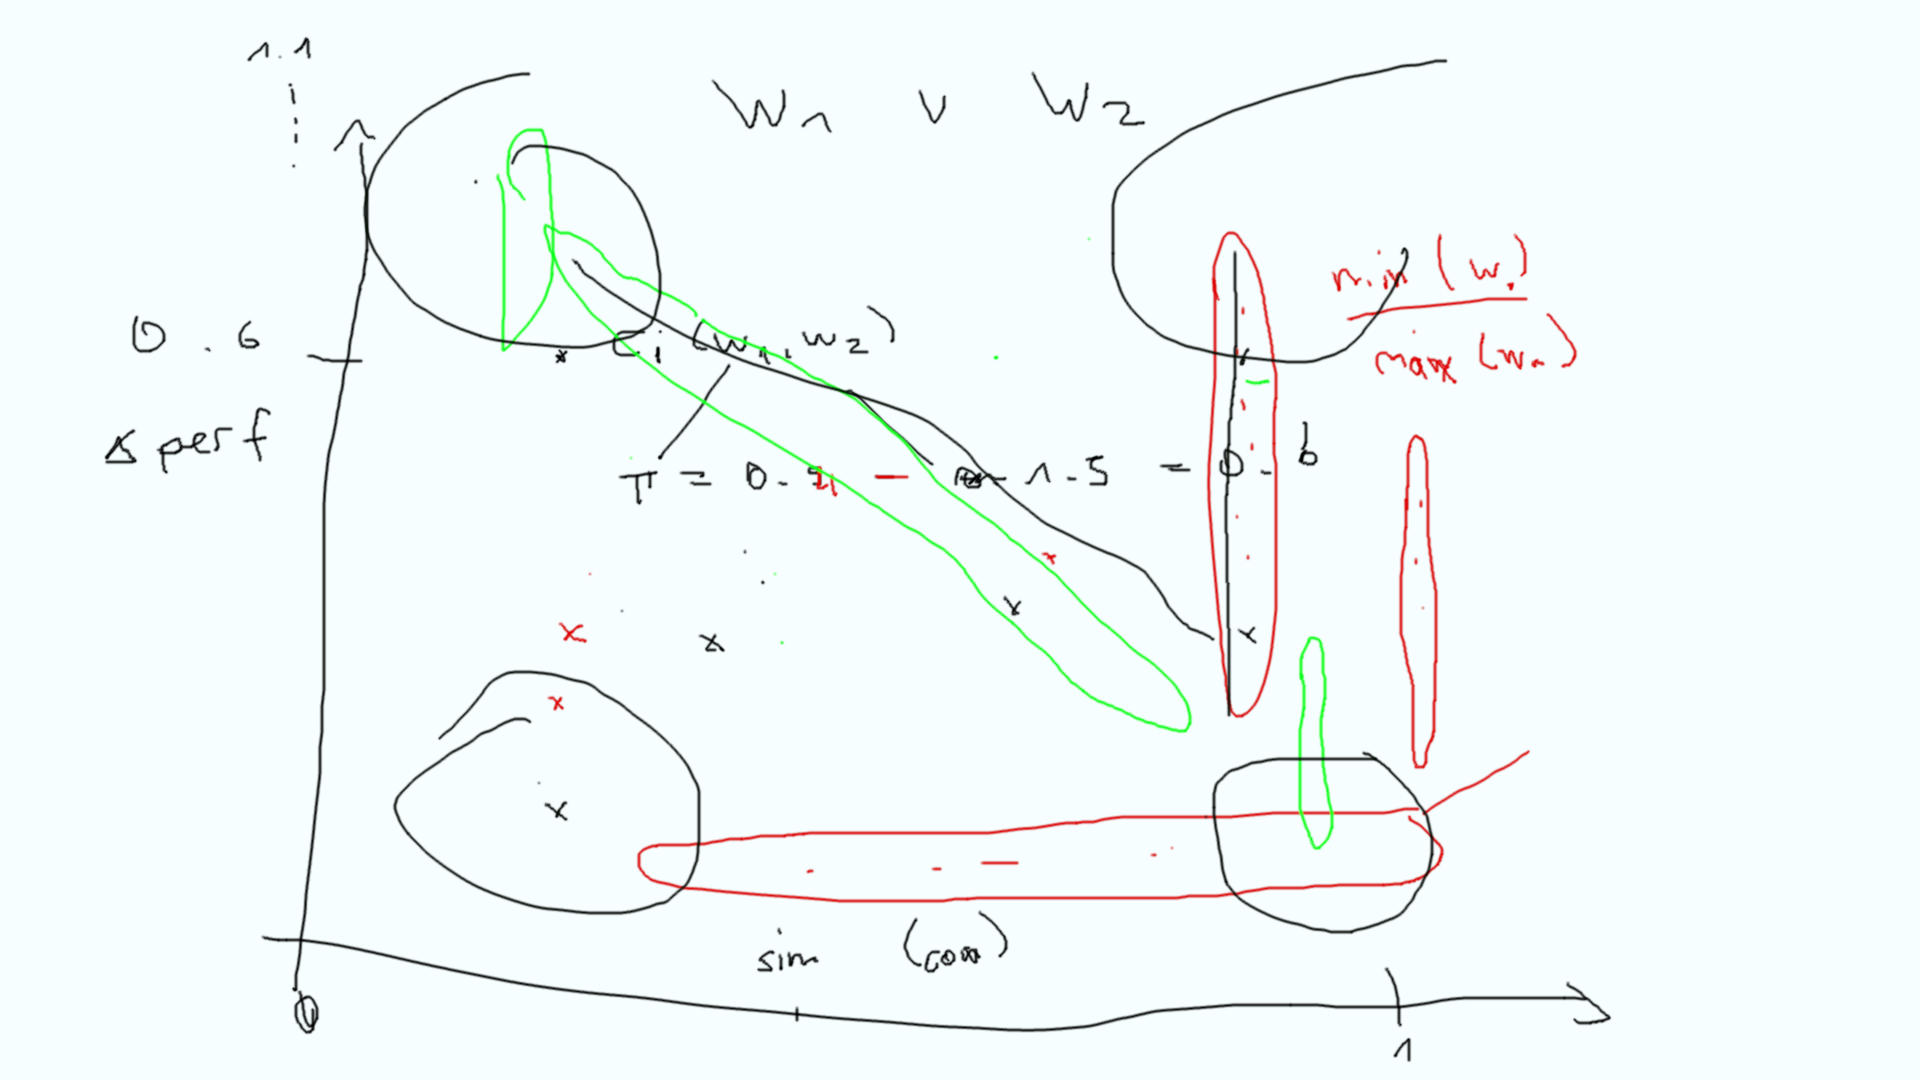
\includegraphics[width=\linewidth]{images/mockup.png}
		\caption{\batik (execution time)}
	\end{subfigure}
	\begin{subfigure}{0.49\textwidth}
		\centering
		%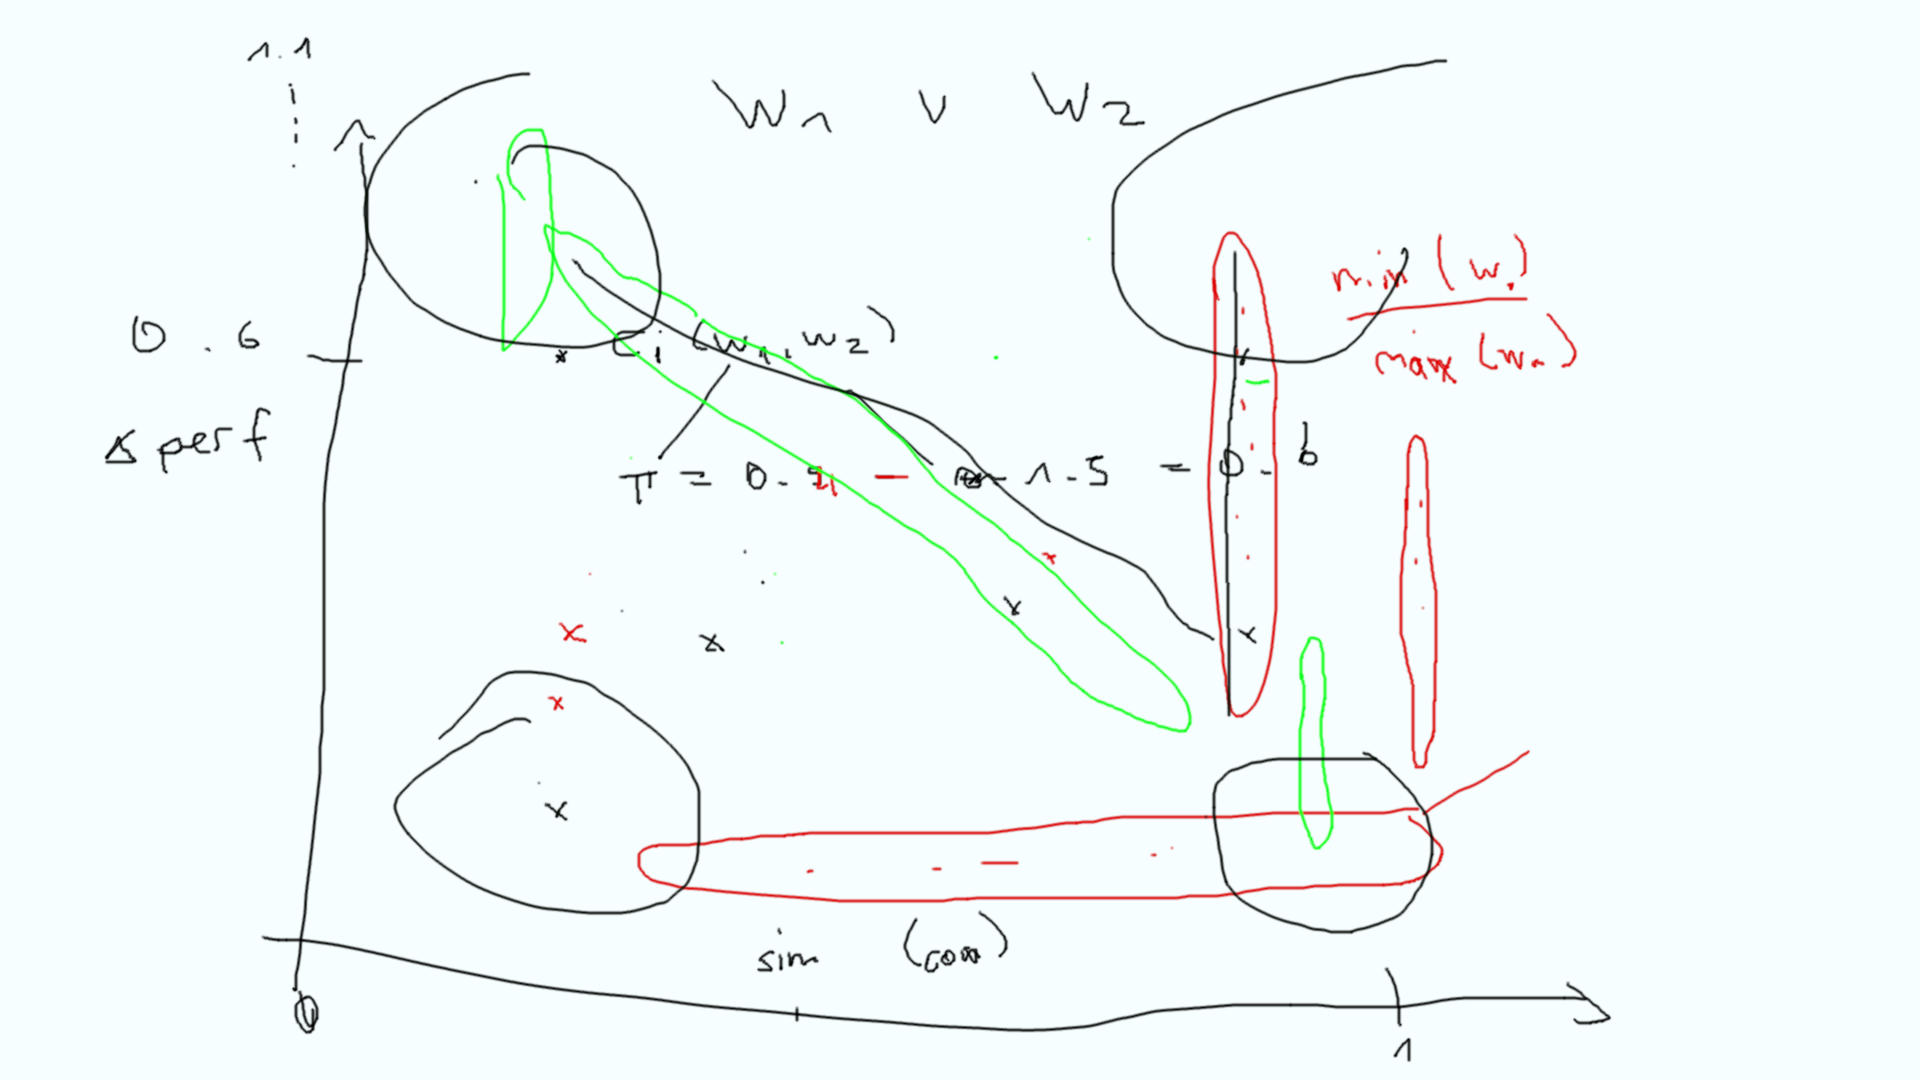
\includegraphics[width=\linewidth]{images/mockup.png}
		\caption{\dconvert (execution time)}
	\end{subfigure}
	\begin{subfigure}{0.49\textwidth}
		\centering
		%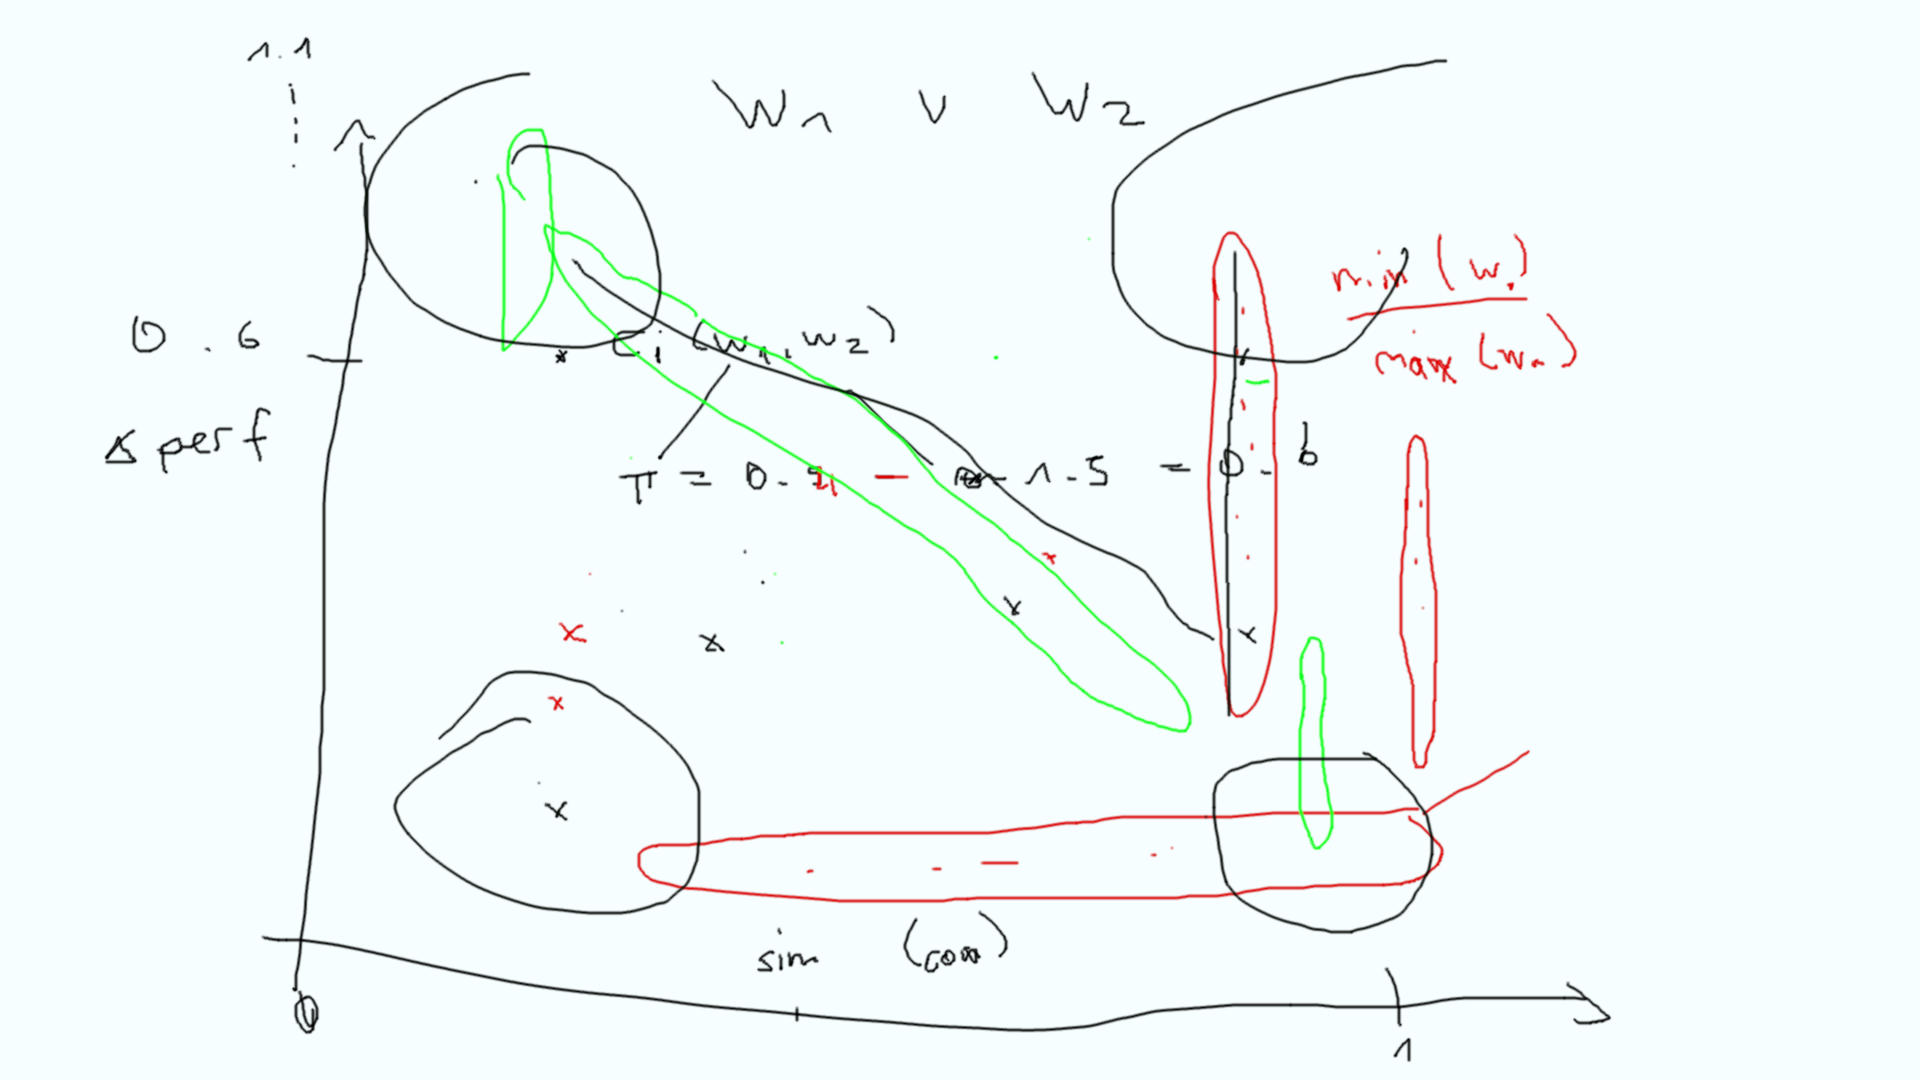
\includegraphics[width=\linewidth]{images/mockup.png}
		\caption{\htwo (throughput)}
	\end{subfigure}
	\begin{subfigure}{0.49\textwidth}
		\centering
		%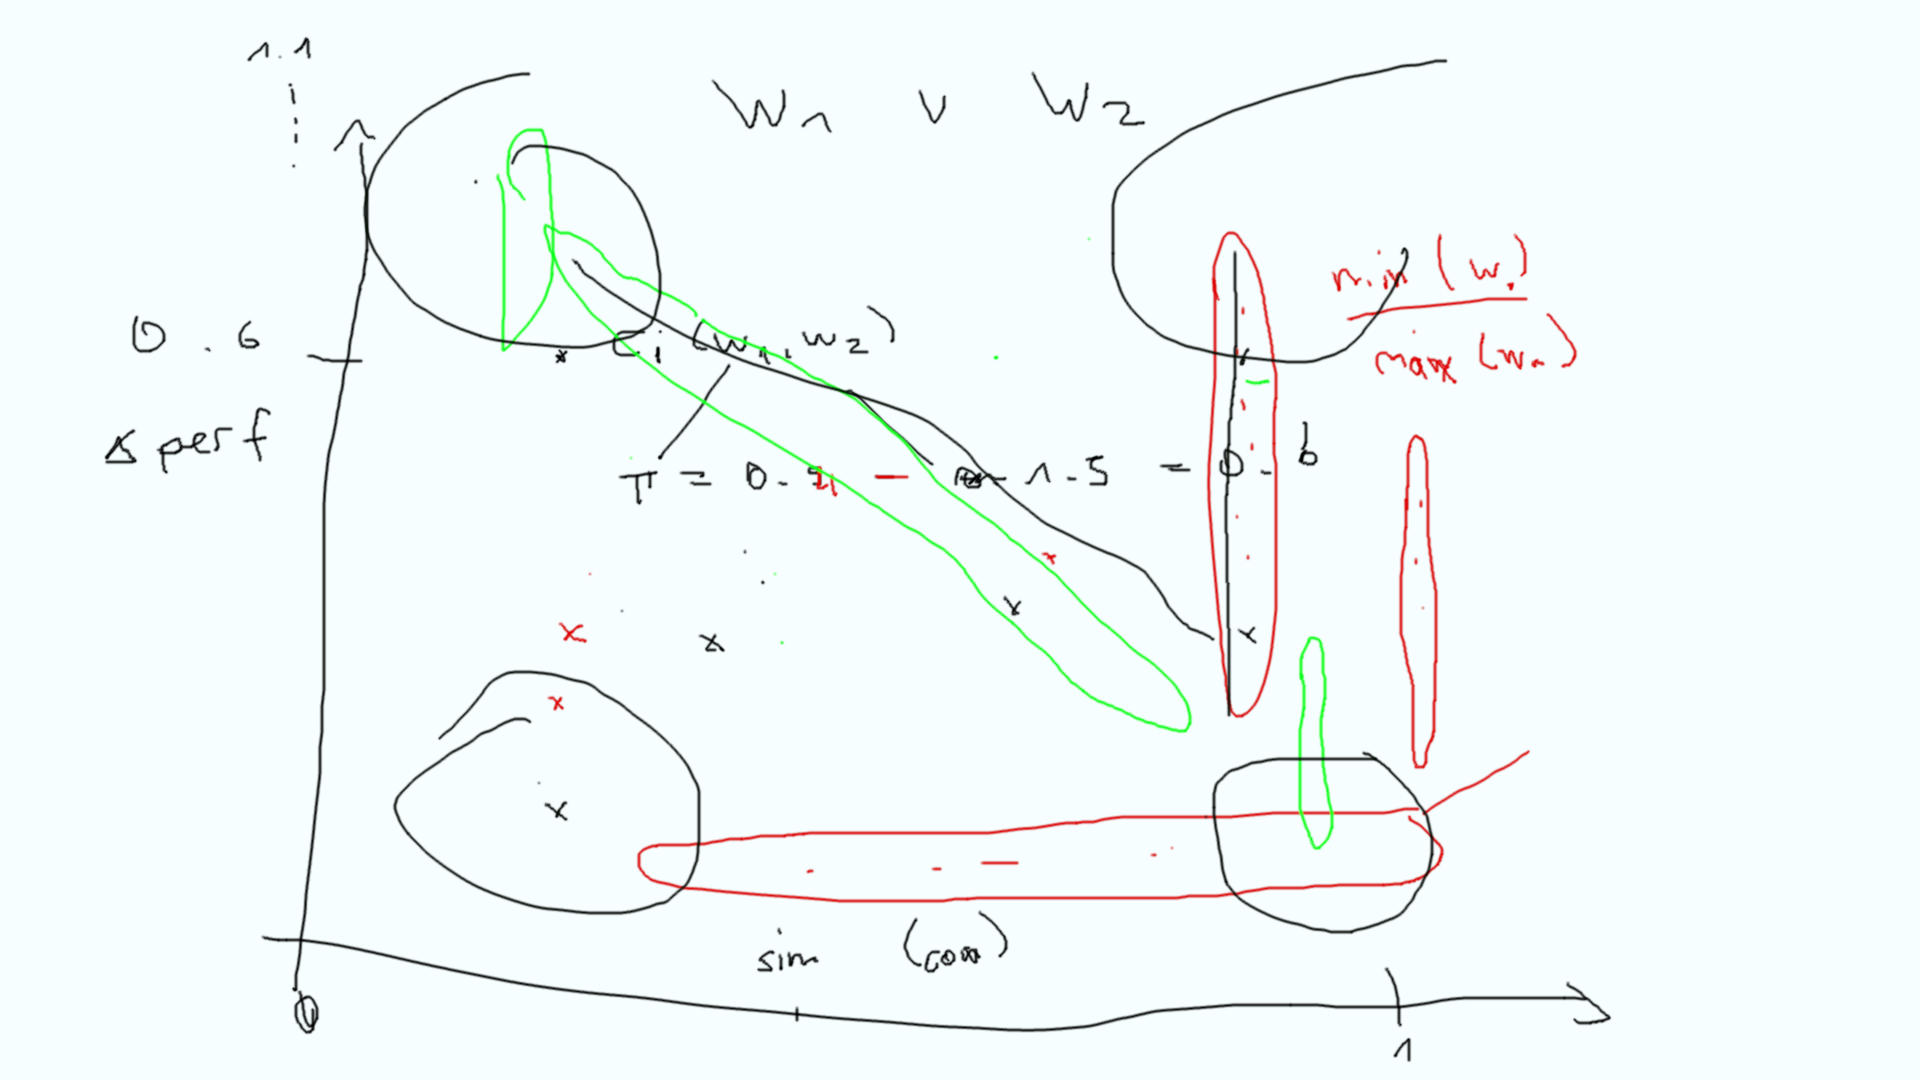
\includegraphics[width=\linewidth]{images/mockup.png}
		\caption{\jumper (execution time)}
	\end{subfigure}
	\begin{subfigure}{0.49\textwidth}
		\centering
		%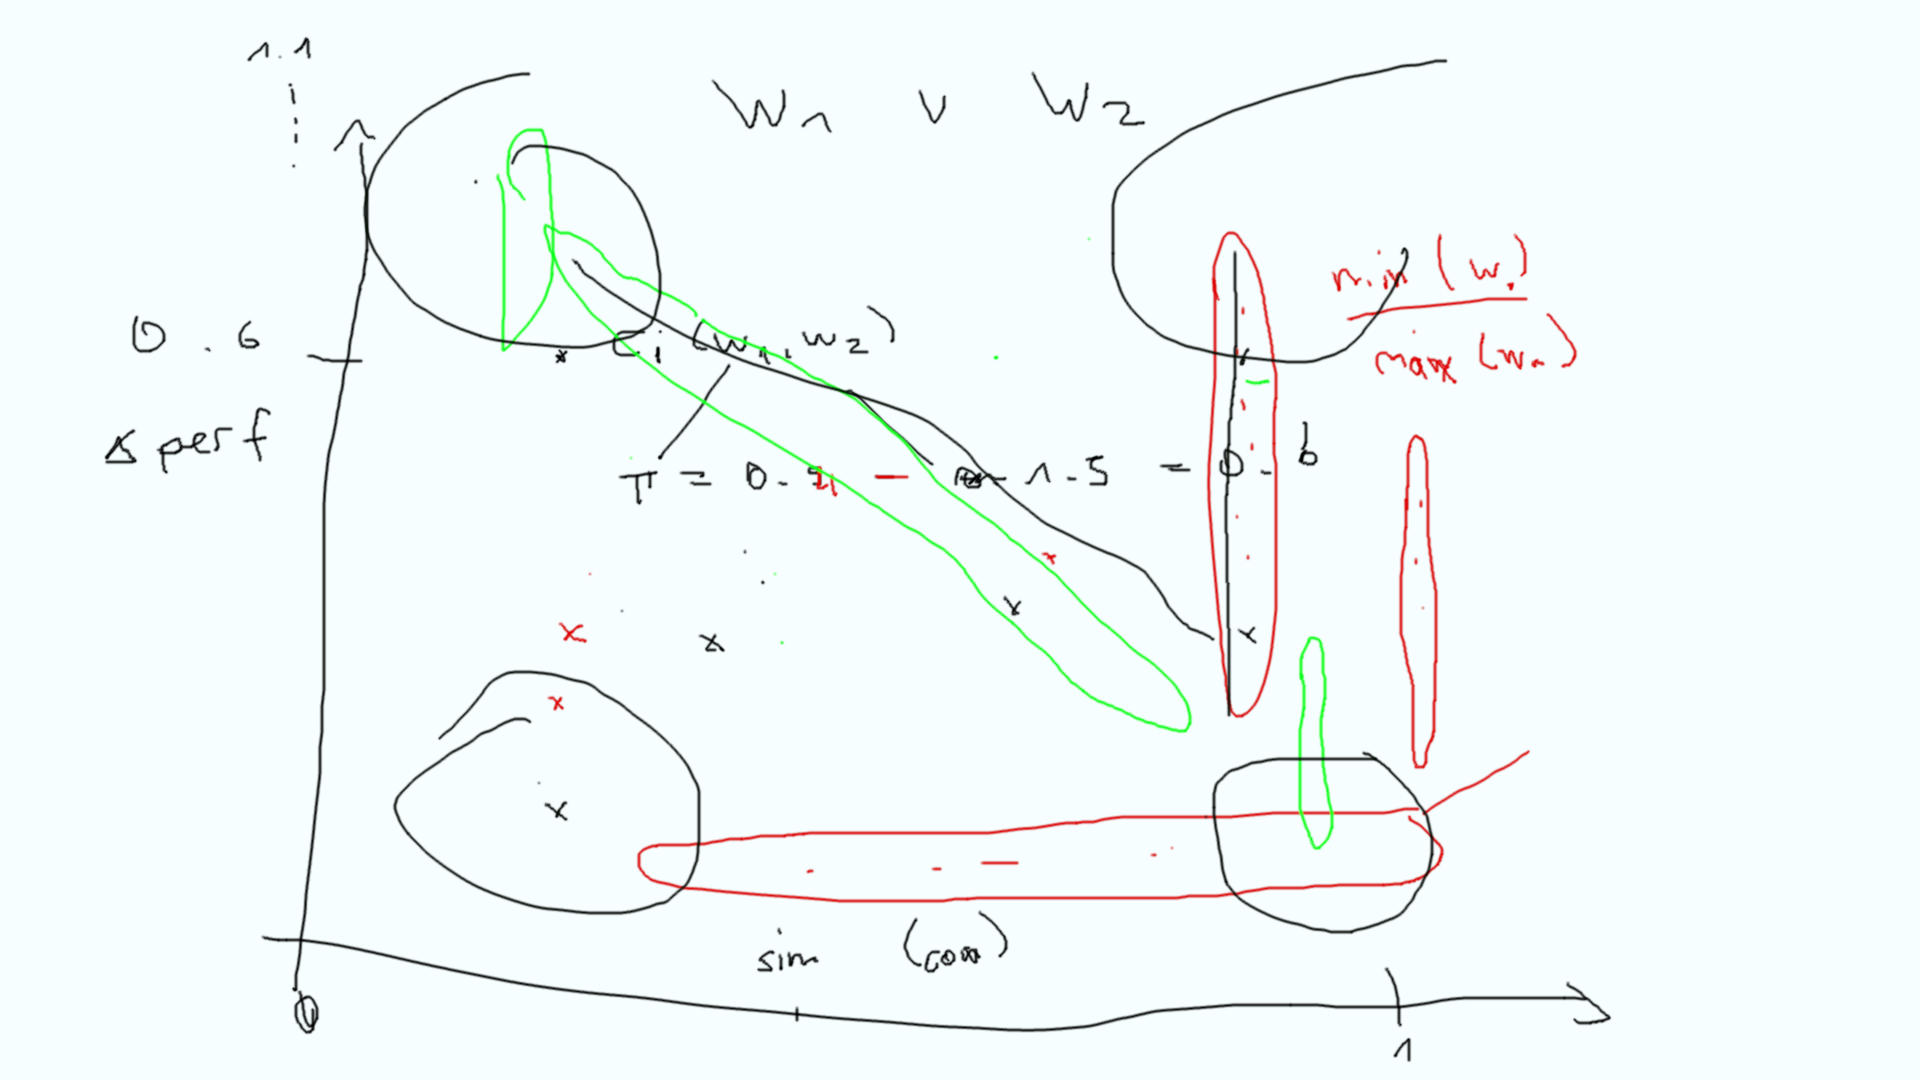
\includegraphics[width=\linewidth]{images/mockup.png}
		\caption{\jadx (execution time)}
	\end{subfigure}
	\begin{subfigure}{0.49\textwidth}
		\centering
		%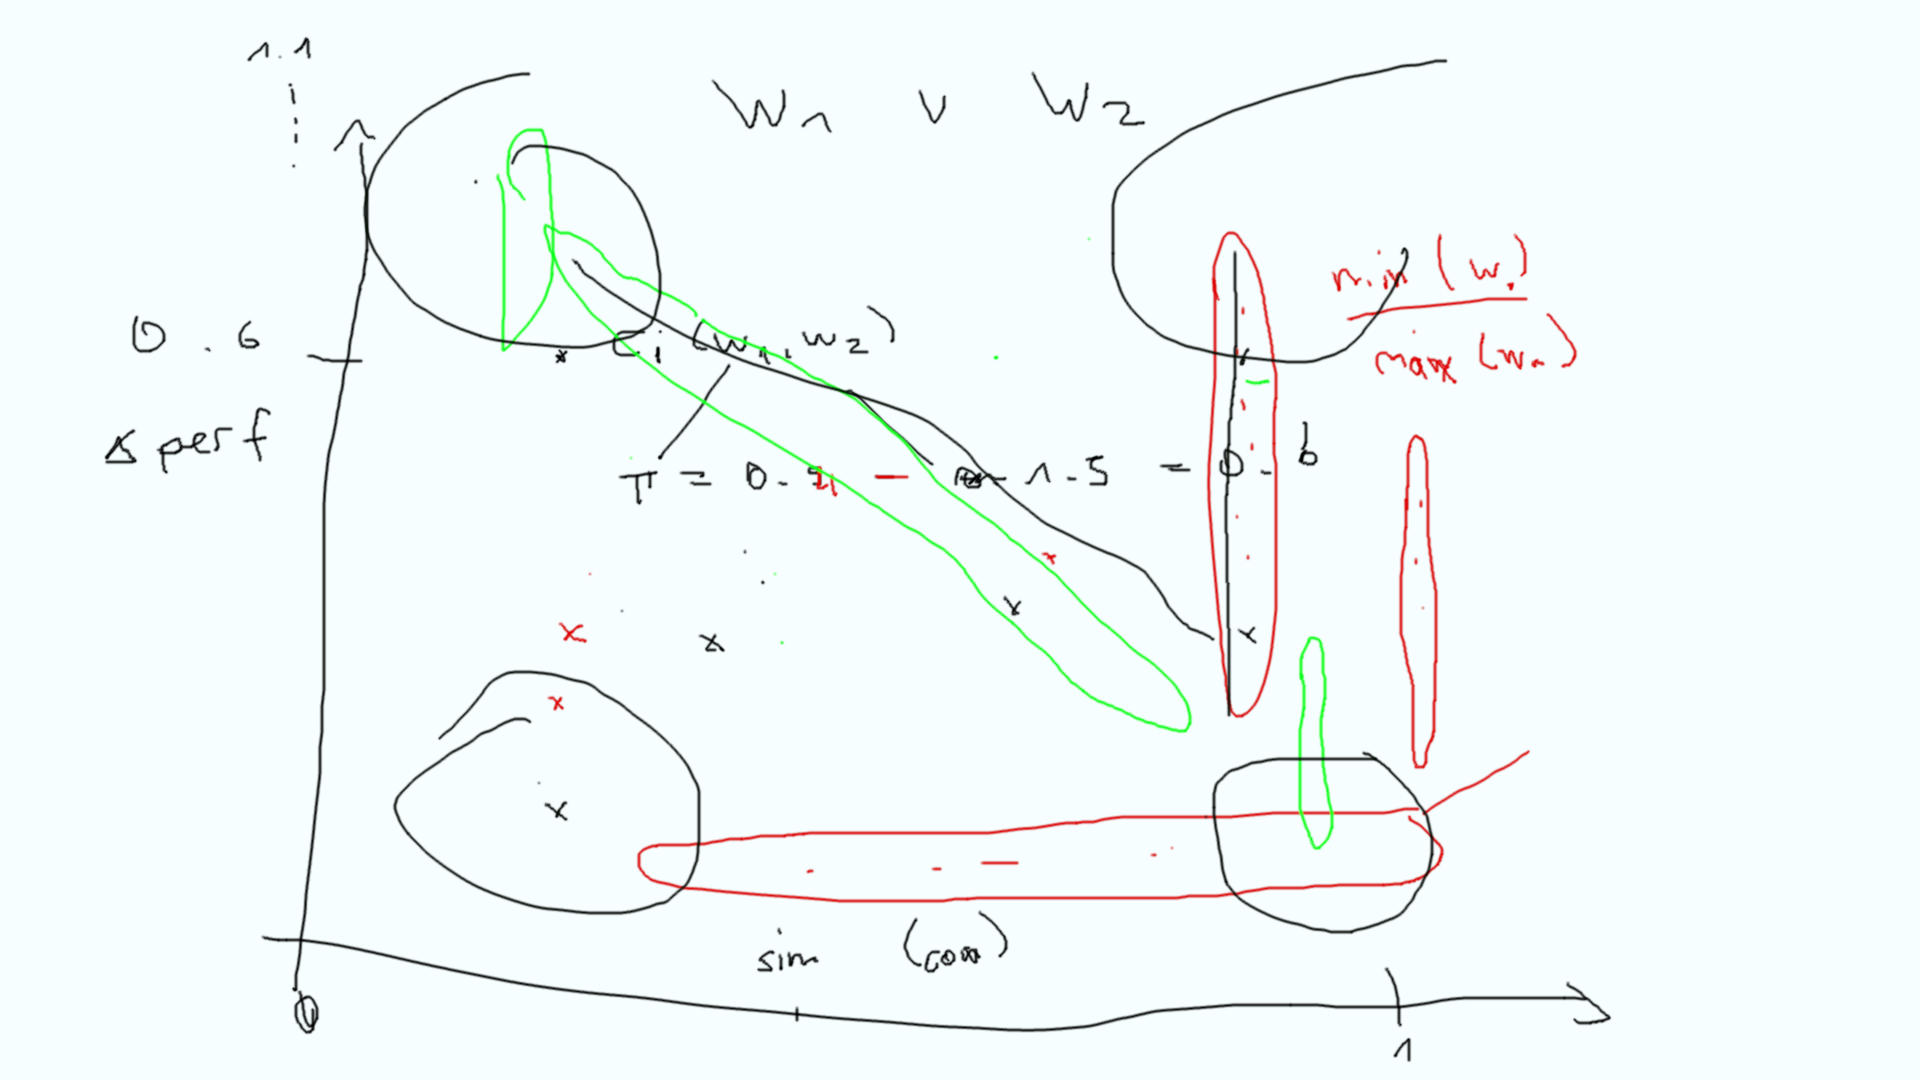
\includegraphics[width=\linewidth]{images/mockup.png}
		\caption{\kanzi (execution time)}
	\end{subfigure}
	\caption{Relationship between differences in configuration code coverage and differences in relative configuration performance for pairs of workloads.}
	\label{fig:diff_config}
\end{figure*}



\paragraph*{Operationalization (RQ~3.2)}
From the results in Figure~\ref{fig:diff_config}, we see that a clear relationship between performance variation and code coverage variation might be rare in practice. However, to deeper investigate the variation in both metrics, we abstract from single configurations to configuration options and relate the performance influences and importances from \RQref{2} with the amount of option-dependent code covered under the respective workloads.

To determine which code can be attributed to a single configuration option or interactions among them, we employ a two-step process. First, we obtain a baseline of all code that depends on a configuration option within the scope of our entire benchmark selection. For each workload $w \in W$, we compute the set of code that depends on option $o \in O$. Let $C_{o}$ be the set of configurations with option $o$ selected, and $C_{\neg o}$ with option $o$ deselected, respectively. To obtain $S_{w, o}$, we follow a strategy similar to spectrum-based feature location~\cite{michelon_spectrum_2021} (cf. Section~\ref{sec:feature_location}) and subtract set of the lines covered under $C_{\neg o}$ from those of $C_{o}$:

\begin{equation}
	S_{w, o} = \bigcup_{p \in C_{o}} S_{w}(p) ~ \setminus ~ \bigcup_{q \in C_{\neg o}} S_{w}(q)
\end{equation}

While $S_{w, o}$ yields an approximation of option-dependent code for a single workload, we aggregate the approximations for each workload $w \in W$ to obtain the set of lines that depend on a configuration option $o$ and are executed in, at least, one workload,~$S_{o}$. 

\begin{equation}
	S_{o} = \bigcup_{w \in W} S_{w, o}
\end{equation}

While this aggregated set should not be mistaken for a ground truth, it enables us to reason about differences in option-dependent code within the scope of our selected workloads. That is, the expressiveness of this baseline depends on the diversity of the workloads in question. We discuss this limitation in Section~\ref{sec:threats}. From the ratio of option-dependent code per workload to option-dependent code across workloads, $\mid S_{w_1, o}\mid/~{\mid S_{w_2, o}\mid}$, we can estimate the coverage of option-dependent code. From comparing the sets $S_{w_1, o}$ and $S_{w_2, o}$ for any two workloads $w_1$ and $w_2$, we can estimate a similarity between the option-code coverage.

\paragraph*{Results}{\color{blue} ... Figure~\ref{fig:diff_performance_option_coverage}}\\

\begin{figure*}
	\centering
	\begin{subfigure}{0.33\textwidth}
		\centering
		(image)
		%\includegraphics[width=\linewidth]{images/mochup_heatmap.png}
		\caption{\batik}
	\end{subfigure}
	\begin{subfigure}{0.33\textwidth}
		\centering
		(image)
		%\includegraphics[width=\linewidth]{images/mochup_heatmap.png}
		\caption{\dconvert}
	\end{subfigure}
	\begin{subfigure}{0.33\textwidth}
		\centering
		(image)
		%\includegraphics[width=\linewidth]{images/mochup_heatmap.png}
		\caption{\htwo}
	\end{subfigure}
	\begin{subfigure}{0.33\textwidth}
		\centering
		(image)
		%\includegraphics[width=\linewidth]{images/mochup_heatmap.png}
		\caption{\jumper}
	\end{subfigure}
	\begin{subfigure}{0.33\textwidth}
		\centering
		(image)
		%\includegraphics[width=\linewidth]{images/mochup_heatmap.png}
		\caption{\jadx}
	\end{subfigure}
	\begin{subfigure}{0.33\textwidth}
		\centering
		(image)
		%\includegraphics[width=\linewidth]{images/mochup_heatmap.png}
		\caption{\kanzi}
	\end{subfigure}
	\caption{Differences in performance influence/importance vs differences in option code coverage}
	\label{fig:diff_performance_option_coverage}
\end{figure*}

\greybox{\textbf{Summary} (\RQref{3.2}):}

\section{Discussion}
\paragraph*{...}
\section{Threats to Validity}\label{sec:threats}

\paragraph*{Internal Validity}\label{sec:internal_validity}
Threats to internal validity include measurement noise which may distort our classification into categories in Section~\ref{sec:rq1} and model construction for Section~\ref{sec:rq2}. We mitigate this threat by repeating each experiment five times and reporting the median as a robust measure. For \htwo, we confirmed a negligible measurement variation in a separate pre-study.
Another potential threat is that the coverage analysis with \mbox{\textsc{JaCoCo}} entails a noticable instrumentation overhead that can distort performance observations. We mitigate this threat by separating the experiment runs for coverage assessment and performance measurement. In the case of \htwo, the load generator of the \textsc{OLTPBench} framework~\cite{difallah_oltp_2013} ran on the same machine as the database since we were testing an embedded scenario, but only introduced negligible variation and overhead.

\paragraph*{External Validity}\label{sec:external_validity}
The selection of subject systems all written in Java poses a threat to external validity. While our motivation for this selection is primarily practical in nature (cf. Section~\ref{sec:setup}), we mitigate this threat by selecting subject systems from variety of domains (cf.~Table~\ref{tab:subject_systems}). Nonetheless, we cannot claim that our results hold for other domains or programming languages. 

In our experiments, we also did not vary the hardware setup for a subject system, which plausibly influences performance as well~\cite{ding_bayesian_2020}, but is beyond the scope of this work. 

\paragraph{Construct Validity}\label{sec:construct_validity}
The profiler \textsc{JaCoCo} instruments Java byte code instructions rather than statements, which leads to some minor imprecision when mapping back covered instructions to the original statements. Transitively, this also affects the precision of our feature location technqiue (cf. Section~\ref{sec:rq3}). This drawback, however, is not limited to this particular profiler, but applies to most profilers operating on byte code. 
The superimposition in our feature location technique is sound, but, by design, incomplete as no set of workloads is guaranteed to cover all feature code. We selected a variety of different workloads, yet our study is of exploratory nature.


\section{Conclusion}
